\documentclass[14pt]{extarticle}
\usepackage[a4paper,				% one-sided article with reduced margins, a4
	    lmargin=2.5cm,rmargin=2cm,		% set left and right margins
	    tmargin=2.5cm,			% set top margin
	    bmargin=2cm,			% set bottom margin
	    marginpar=1cm,			% set margin notes width
	    marginparsep=0.5cm,			% set notes to paragraph separation width
headheight=17pt]{geometry} % set head height
 
%Russian-specific packages
%--------------------------------------
\usepackage[T2A]{fontenc}
\usepackage[utf8]{inputenc}
\usepackage[russian]{babel}
%--------------------------------------
\usepackage[paper=portrait,pagesize]{typearea}
\usepackage{graphicx}
\usepackage{lastpage}


\begin{document}

\begin{center}

    Министерство образования и науки Российской Федерации\\
    Федеральное государственное бюджетное образовательное учреждение высшего образования\\
    Волгоградский государственный технический университет\\
    Кафедра <<Системы автоматизированного проектирования и поискового конструирования>>
\end{center}
\vspace{70pt}
\begin{flushright}

    УТВЕРЖДАЮ\\
    Зав. кафедрой САПР и ПК\\
    \rule{25mm}{0.4pt} д.т.н. Щербаков М. В.\\
    <<\rule{7mm}{0.4pt}>> \rule{35mm}{0.4pt} 2018 г
\end{flushright}

\begin{center}
    \LargeРазработка программы для подготовки трудового договора и отчёта по второму высшему образованию\\
    \vspace{30pt}
    \normalsizeТЕХНИЧЕСКОЕ ЗАДАНИЕ\\
    Листов - \pageref{LastPage}\\
    \vspace*{\fill}
    Волгоград, 2018г.\\
\end{center}

\newpage
 
\tableofcontents
\newpage

\section{Введение}
    \subsection{Наименование программы}
    Наименование – «Программа для подготовки трудового договора и отчёта по второму высшему образованию». \\Краткое наименование – программа.
    \subsection{Краткая характеристика области применения}
    Разрабатываемая программа предназначена для применения на кафедре САПР и ПК ВолгГТУ и должна служить эффективным инструментом для составления трудовых договоров.
 
\section{Основания для разработки}
    \subsection{Документы, на основе которых ведётся проектирование}
    В качестве лабораторной работы №5 по курсу «Проектирование АСОиУ» было получено задание на проектирование программы, осуществляющей подготовку трудового договора по второму высшему образованию.
    \subsection{Организация, утвердившая документ, и дата утверждения}
    Документ утвердил д.т.н., зав. кафедрой САПР и ПК Щербаков М. В.\\
    Дата утверждения документа: <<\rule{7mm}{0.4pt}>> \rule{35mm}{0.4pt} 2018 г
    \subsection{Наименование темы разработки}
    Тема разработки – «Разработка программы для подготовки трудового договора и отчёта по второму высшему образованию».
    
\section{Назначение разработки}
Разрабатываемая программа предназначена для формирования трудового договора и отчёта по второму высшему образованию.

\section{Требования к программе}
    \subsection{Требования к функциональным характеристикам}
        \subsubsection{Требования к составу выполняемых функций}
        Программа должна обеспечивать конечному пользователю возможность выполнения перечисленных ниже функций:\\
        - получение данных:\\
            \hspace*{3em} - получение информации из расписания семестра о читаемых дисциплинах и ответственных за это преподавателях;\\
            \hspace*{3em} - получение информации из списков групп (количество студентов);\\
            \hspace*{3em} - получение информации о совмещаемых предметах с кафедрой ЭВМ и С;\\
            \hspace*{3em} - получение информации о стоимости часа в текущем учебном году;\\
            \hspace*{3em} - получение данных о переаттестациях студентов;\\
            \hspace*{3em} - получение персональных данных преподавателя;\\
            \hspace*{3em} - получение формулы для расчёта заработной платы из приказа <<О нормах времени>>;\\
        - расчёт заработной платы преподавателя на основе формул и собранных данных;\\
        - занесение полученной информации в договор.\\
       
        \subsubsection{Требования к организации входных данных}
        На вход программы должны быть переданы следующие входные данные.\\
        Информация о читаемых дисциплинах и ответственных за это преподавателях должна подаваться на вход программы в виде таблицы.\\
        Информация о количестве студентов в группах должна подаваться в виде списка группы.\\
        Информация о совмещаемых дисциплинах с кафедрой ЭВМ и С должна быть представлена в виде документа в формате .docx.\\
        Информация о стоимости часа содержится в соответствующем приказе, который должен быть предоставлен программе в формате .docx.\\
        Данные о переаттестации студентов должны быть поданы на вход программы в виде соответствующего документа в формате .docx.\\
        Персональные данные преподавателя должны иметь возможность быть выбранными из выпадающего списка, который администратор заранее должен заполнить данными всех преподавателей кафедры.\\
        Формула для расчёта заработной платы должна подаваться на вход программы в составе соответствующего приказа «О нормах времени» в формате .docx.\\
        Все необходимые документы должны быть упакованы в одну папку и иметь названия, по которым программа сможет самостоятельно к ним обратиться.\\
        
        \subsubsection{Требования к организации выходных данных}
        Выходные данные должны быть представлены сформированным трудовым договором в формате .docx.
        
    \subsection{Требования к надёжности}
        \subsubsection{Требования к обеспечению надёжного функционирования программы}
        Надежное функционирование программы должно быть обеспечено совокупностью организационно-технических мероприятий, перечень которых приведен ниже:\\
        -	организацией бесперебойного питания технических средств;\\
        -	использованием лицензионного программного обеспечения.
        
        \subsubsection{Время восстановления после отказа}
        Время восстановления после отказа, вызванного сбоем электропитания технических средств (иными внешними факторами), не фатальным сбоем (не крахом) операционной системы, не должно превышать времени, требуемого на восстановление подачи электропитания и запуск программы.\\
        Время восстановления после отказа, вызванного неисправностью технических средств, фатальным сбоем (крахом) операционной системы, не должно превышать времени, требуемого на устранение неисправностей технических средств, и переустановки программных средств.
        
        \subsubsection{Отказы из-за некорректных действий оператора}
        Отказы программы возможны вследствие некорректных действий оператора (пользователя) при взаимодействии с операционной системой. Во избежание возникновения отказов программы по указанной выше причине следует обеспечить работу конечного пользователя без предоставления ему административных привилегий.
        
    \subsection{Условия эксплуатации}
        \subsubsection{Требования к численности и квалификации персонала}
        Минимальное количество персонала, требуемого для работы программы должно не менее 2 штатных единиц – системный администратор и конечный пользователь программы.\\
        Системный администратор должен иметь высшее профильное образование и сертификаты компании-производителя операционной системы. В перечень задач, выполняемых системным администратором, должны входить:\\
        -	задача поддержания работоспособности технических средств;\\
        -	задачи установки (инсталляции) и поддержания работоспособности системных программных средств – операционной системы.

    \subsection{Требования к составу и параметрам технических средств}
    Состав технических средств, а также общесистемного и прикладного программного обеспечения программы:\\
    - операционная система Microsoft Windows XP и старше;\\
    - процессор Intel Pentium 4 или AMD Athlon с тактовой частотой выше 1.4 ГГц;\\
    - ПЗУ на 1Гб;\\
    - объем свободной оперативной памяти – 1 Гб;\\
    - видеоадаптер SVGA, монитор, поддерживающий режим работы SVGA; \\
    - клавиатура, мышь.

    \subsection{Требования к информационной и программной совместимости}
        \subsubsection{Требования к методам решения}
        
        Данные методы решения должны обеспечивать выполнение всех этапов проектирования программы в соответствии с их порядком и сроками выполнения, указанными в разделе 6 данного документа.
        \subsubsection{Требования к исходным кодам и языкам программирования}
        Программа должна быть реализована на базе платформы 1с с применением встроенного языка программирования.
        
    \subsection{Требования к программным средствам, используемым программой}
    Системные программные средства, используемые разрабатываемой программой, должны быть представлены лицензионной локализованной версией операционной системы, а также платформой 1с.
    
\section{Требования к программной документации}
    \subsection{Состав программной документации}
    Состав программной документации должен включать в себя техническое задание на разработку и проектирование программы (ГОСТ 19), пояснительную записку, руководство пользователя и исходные коды программы.
    
\section{Стадии и этапы разработки}
Проектирование программы должно включать в себя стадии, приведённые в Таблице 1.\\
\begin{table}[h!]
\caption{Сроки выполнения работ}
    \begin{center}
    
    \label{tab:table1}
      \begin{tabular}{|c|c|c|}
      \hline
№ п/п & Наименование стадии             & Сроки         \\
\hline
1     & Анализ требований пользователя  & 6/11/2018     \\
\hline
2     & Разработка технического задания & 14/11/2018     \\
\hline
        \end{tabular}
        \end{center}
\end{table}

\section{Порядок контроля и приёмки}
    \subsection{Виды испытаний}
    Приёмо-сдаточные испытания должны проводиться не ранее окончания реализации программного продукта.
    \subsection{Общие требования к приёмке работы}
    Возможность приёмки программы должна определяться соответствием всем пунктам настоящего технического задания.

\newpage

 \\
 \\
\KOMAoptions{paper=landscape,pagesize}
\section*{Приложение А. BPMN диаграмма процесса}
\addcontentsline{toc}{section}{Приложение А. BPMN диаграмма процесса}
%\recalctypearea

\begin{landscape}\centering
\begin{figure}[h!]
  \centering
  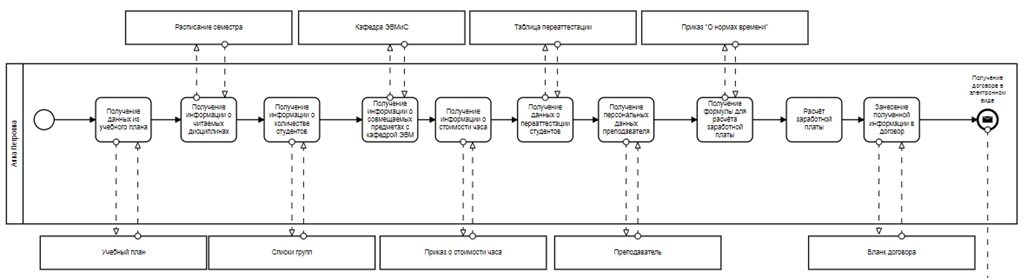
\includegraphics[width=1.5\textwidth]{BPMN1.jpg}
  \caption{Functional Decomposed Data Structure}
\end{figure}
\vfill
\end{landscape}

\newpage

\begin{figure}[h!]
 \centering
 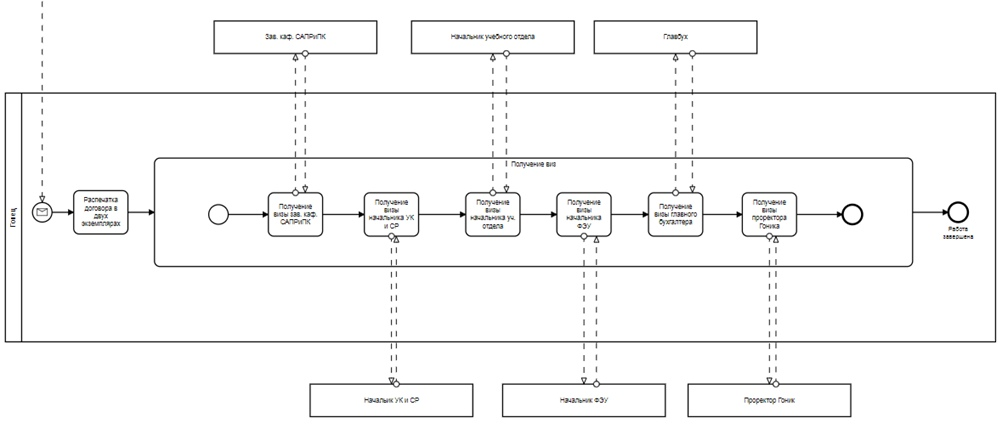
\includegraphics[width=1.5\textwidth]{BPMN2.jpg}
\end{figure}
 
\end{document}

% 
% 